\section{Memory}
%---------------------------

Logic circuits need to store the numbers they are working with in order to do more than one thing. Central Processing Units (CPUs), Arithmetic Logic Units (ALUs) or Floating-Point Units (FPUs) each work with numbers, and need to fetch them from somewhere and put them somewhere when they are done. The ``somewhere" is \emph{memory}. Keeping with the use of binary math and binary logic, a high voltage would be a 1 and a low voltage would be a 0. Through the use of these little stored charges, computers can keep track of many, many pieces of information. No matter what the circuits are doing, everything being stored is composed of some count of zeros and ones. 

There have been \emph{many} forms of memory through the years, including punched paper cards, and even a wiggly wire! The most common memory that a CPU uses these days is usually called ``dynamic RAM" (DRAM), and each bit consists of a circuit that is primarily a single capacitor and a single transistor, though it requires supporting circuitry and cannot be read without erasing the memory cell. Computers read eight, sixteen, 32, or 64 bits at a time from a row of memory and pass the information (numbers or instruction codes) from the memory on to be processed by the CPU.

One type of computer memory, called \emph{static RAM}, uses at least six transistors per bit. Since  DRAM is simpler (it uses only one transistor and one capacitor per bit), it is also cheaper. Therefore, to store one bit with 6 or more transistors is more expensive. So SRAM is mostly used for very important memory, like the memory very close to the core of the computer processor. Have a look at Figure \ref{fig:sram}\footnote{Diagram and supporting information adapted from {\color{webblue}\href{https://en.wikipedia.org/wiki/Static_random-access_memory}{Wikipedia}} and {\color{webblue}\href{https://www.entner.net/sites/default/files/diss-entner-final-v1.pdf}{Robert Entner's dissertation}}.}, 
which is pretty complicated, but if you understand how the two types of transistors are turned on and off, it will make sense. To keep this diagram simple, no resistors are shown. If you look closely at the $Q_1$/$Q_2$ and $Q_3$/$Q_4$ transistors, you can see that they are acting like inverters (that is, each pair makes a NOT gate). When WL (the ``word line") goes high, $Q_5$ and $Q_6$ open up, allowing access to the single bit stored in $BL$ and the inverse of that bit in $\overline{BL}$. Whether the word line is active (that is, whether or not you can write to the memory bit), it is possible to read the value of the bit--making SRAM very fast, because the system does not wait on the word line to activate.


\begin{figure}[h!]
\begin{center}
\newcommand*\low[1]{\overline{#1}}

\begin{circuitikz}

\draw 
% Vdd:
%	(4,5) node[vdd](vdd){}
	(2,5) node[circ](vdd1) {}
	(6,5) node[circ](vdd2) {}	
    (4,5) node[above] {{\color{red}$V_{dd}$}} % Vdd
    (1.5,5) |- (6.5,5)

% GND
	(2,0) node[circ](gnd1) {}
	(6,0) node[circ](gnd2) {}
    (4,0) node[ground](ground){}
    (1.5,0) |- (6.5,0)
;


% Bit Line nodes:
\draw
	(0,2.25) node[circ, color=blue](bllow) {}
	(0,1) node[left] {{\color{red}$\low{BL}$}} % BL low
;

\draw
	(8,2.75) node[circ, color=orange](blhigh) {}
	(8,1) node[right] {{\color{red}$BL$}} % BL
;

% Bit Line:
\draw[blue, thick]
	(0,0) |- (0,6)
;

% Bit Line Complement:
\draw[orange, thick]
	(8,0) |- (8,6)
;


% Word Line nets and nodes:
\draw[green!70!black, thick]
	(1,6) node[circ, color=green!70!black](wlgate1){} 
	(4,6) node[above] {{\color{red}$WL$}} % WL label
	(0.5,6) |- (7.5,6)

	(7,6) node[circ, color=green!70!black](wlgate2){}
;

\draw
% Two inverters:

% 2 P-type FETs:
	(2,4) node[pmos, emptycircle, xscale=-1](Q2){}
	(1.5,4) node[above]{$Q_2$}
	(6,4) node[pmos, emptycircle](Q4){$Q_4$}


% 2 N-type FETs:
	(2,1) node[nmos, xscale=-1](Q1){}
	(1.5,1) node[above]{$Q_1$}
	(6,1) node[nmos](Q3){$Q_3$}


% Word line gate N-type FETs:
	(1,2.25) node[nmos, rotate=-90](Q5){}
	(0.5,3.0) node[above]{$Q_5$}
	
	(7,2.75) node[nmos, rotate=-90](Q6){}
	(7.5,3.45) node[above]{$Q_6$}
;


% Inverter net intersection nodes:
\draw[green!70!black, thick]
 (6, 2.75) node[circ, color=red!30!blue!90] (m6Q1){}
 (2, 2.25) node[circ, color=red] (m5Q1){}
;
 

 
\draw
 (2.98,2.75) node[circ, color=red!30!blue!90] (m6q2){}
 (5.01,2.25) node[circ, color=red] (m5q2){}
;


% Nets:

\draw[green!70!black, thick]
 (wlgate1) |- (Q5.G)
 (wlgate2) |- (Q6.G)
;

\draw
 (vdd1) |- (Q2.S)
 (vdd2) |- (Q4.S)

 (Q1.S) |- (gnd1)
 (Q3.S) |- (gnd2)
;

\draw[red, thick]
 (Q1.D) |- (Q2.D)
;

\draw[red!30!blue!90, thick]
 (Q3.D) |- (Q4.D)
 (Q2.G) |- (Q1.G)
 (Q6.S) |- (2.97,2.75)
;

\draw[red, thick]
 (Q4.G) |- (Q3.G)
 (Q5.D) |- (5.01,2.25)
;

\draw
 (bllow) |- (Q5.S)
 (blhigh) |- (Q6.D)
;

\end{circuitikz}
\caption{A static ram cell. The bit line ($BL$) on the right is the value of the bit, and the bit line on the left ($\low{BL}$) is the complement (NOT) the value of that bit.} % With a bit of careful circuitry, it is possible to write using only one of the bit lines, but it is safer to have two inputs (one positive, and one complement) to ensure the gates both change and lock in the value of the bit.  
\label{fig:sram}
\end{center}
\end{figure}

SRAM uses 6 transistors per bit, making it very expensive compared to dynamic RAM, 
but each bit of SRAM can stand alone, with no other supporting circuitry except 
for the word line transistors. So, we use SRAM here because you can see the 
circuit, and see how it works. As a bonus, you can construct a bit of SRAM with 
opposing NOT gates, making it fairly easy to see what is happening.

\begin{figure}
  \begin{center}
  %\documentclass[12pt]{article}
%\usepackage[left=1in,right=1in,top=1in,bottom=1in]{geometry} 
%\usepackage{xcolor}
%\usepackage{tikz}
%\usepackage[american, EFvoltages, cuteinductors]{circuitikz}
%
%\begin{document}
%\thispagestyle{empty}
%
%\begin{figure}[h!]
%\begin{center}
%
\begin{circuitikz}


% Clock input:
\draw
	(-2cm,2.75cm) node[ocirc](clknode) {} % CLK node
	node[left] {{\color{red}$CLK$}} % CLK label
;


% Inputs and 3-input NAND gates:
\begin{scope}
	\draw
		(0,4.25) 
		node[american nand port, anchor=in 2, number inputs = 3](J){}
		node[ocirc, xshift = -2cm](jnode){}
    	node[xshift = -2cm, yshift = 3mm](){{\color{red}$J$}}
		node[xshift = 0.9cm, yshift = 1.0cm] {{\footnotesize{$NAND_1$}}} 
		(jnode) |-  (J.in 2)
	;

	\draw
		(0,1.75) 
		node[american nand port, anchor=in 1, number inputs = 3](K){}
		node[ocirc, xshift = -2cm, yshift = -4mm](knode){}
    	node[xshift = -2cm, yshift = -1mm](){{\color{red}$K$}}
		node[xshift = 0.9cm, yshift = -1.3cm]{{\footnotesize{$NAND_2$}}} 
		(knode) |-  (K.in 2)
	;
\end{scope}


% Q output:
\draw
    (5,3.97) 
	node[american nand port] (Nand3){}
	node[xshift = -5mm, yshift = 1.0cm]{{\footnotesize{$NAND_3$}}} 
	node[ocirc, xshift=2cm, yshift=0mm](qnode){}
	node[xshift = 2cm, yshift = 3mm](){{\color{red}$Q$}}
	(Nand3.out) to (qnode)
;


% not-Q output:
\draw
	(5,1.65) node[american nand port] (Nand4){}
	node[xshift = -5mm, yshift = -1.0cm] {{\footnotesize{$NAND_4$}}} 
	node[ocirc, xshift=2cm, yshift=0mm](notqnode){}
	node[xshift = 2cm, yshift = 4mm](){{\color{red}$\overline{Q}$}}
	(Nand4.out) to (notqnode)
;


% Nets and labels from the three-input NANDs to the SR circuit:
\draw(J.out) -| (Nand3.in 1);
\draw(K.out) -| (Nand4.in 2);

\draw
	(Nand3.in 1)
	node[yshift = 3mm, xshift = -2mm](nots){{\color{red}$\overline{S}$}}
;

\draw
	(Nand4.in 2)
	node [yshift = -3mm, xshift = -2mm](notr){{\color{red}$\overline{R}$}}
;


% Shaded box surrounding the basic SR Flip-Flop:
\filldraw (5cm,2.8cm) node[minimum size=5cm, draw, fill=blue!40, opacity=0.3]{};


% Clock input line nets:
\draw[blue, thick]
	(-0.5, 2.75) node[circ, color=blue](clknode2){}
	(clknode) to (clknode2)
	(clknode2) |- (J.in 3)
	(clknode2) |- (K.in 1)
;

% Signal / feedback from NAND outputs to 3-input NAND inputs and SR NAND inputs:
\draw (Nand4.in 1)--++(180:5mm)--++(90:3mm)--([yshift=-3mm] Nand3.out)--(Nand3.out);
\draw (Nand3.out) node[circ ](aux3){};

\draw (Nand3.in 2)--++(180:5mm)--++(-90:3mm)--([yshift=3mm] Nand4.out)--(Nand4.out);
\draw (Nand4.out) node[circ ](aux4){};

\draw (Nand4.out) node[circ, xshift = 5mm](aux1){};
\draw (aux1) --++(90:4cm)--++(-180:3cm) -| (J.in 1);

\draw (Nand3.out) node[circ, xshift = 8mm](aux2){};
\draw (aux2) --++(-90:4cm)--++(-180:3cm) -| (K.in 3);


\end{circuitikz}

%\caption{A gate-level schematic of one bit of memory, using a JK flip-flop circuit.}
%\end{center}
%\end{figure}

%\end{document}

  \caption{A gate-level schematic of one bit of memory, using a JK flip-flop circuit. Note that the two left-most NAND gates have \emph{three} inputs.}
  \end{center}
\end{figure}

% JK flip-flop: 
% Flip-flop storage using NOR gates is better than my previous attempt using NOT gates. 
% I had trouble with the word/line controller circuit resistor values for positive 
% clearing and setting of the gate states. 

We are going to implement some RAM using a {\color{webblue}\href{https://www.electronics-tutorials.ws/sequential/seq_2.html}{\emph{flip-flop}}} circuit, made of NAND gates.
It uses even more transistors than the SRAM circuit, but it is simpler to create and uses logic gates with which you are already familiar. This ``JK Flip-Flop" circuit uses
two input NAND gates and also \emph{three}-input NAND gates. 3-input NAND operates mostly
the same way as a regular NAND gate, except that the inputs also include the value of the 
Q and not-Q output (value) lines. 
These lines are required before the output state (value) of the gate will change. And so is a ``clock" signal line. By using a signal that turns on or turns off everywhere at once, the computer memory can be more reliable. The clock line ticks on and off like the second hand of a clock, allowing the computer to read or write to the memory without wondering if the values are changing.
So, the set- and reset- functions for the memory cell
only activate when the clock signal is also high (has positive voltage on the line).
This extra feature allows for certainty of reads and writes: it helps
avoid rapid oscillation / instability or lock-ups should a circuit (or a third
grader!) try to both set and reset the
flip-flop at the same time. Furthermore, when powering up a simple SR flip-flop,
there is no inherent guarantee of what the value would be (of course, it's
possible to put a pull-up or pull-down resistor on the signal lines to create
a natural ``base level'' of a set of inputs, though care must be taken to 
not accidentally create incompatible base conditions (such as accidentally setting
both set and reset to high).

\begin{figure}
  \begin{center}
    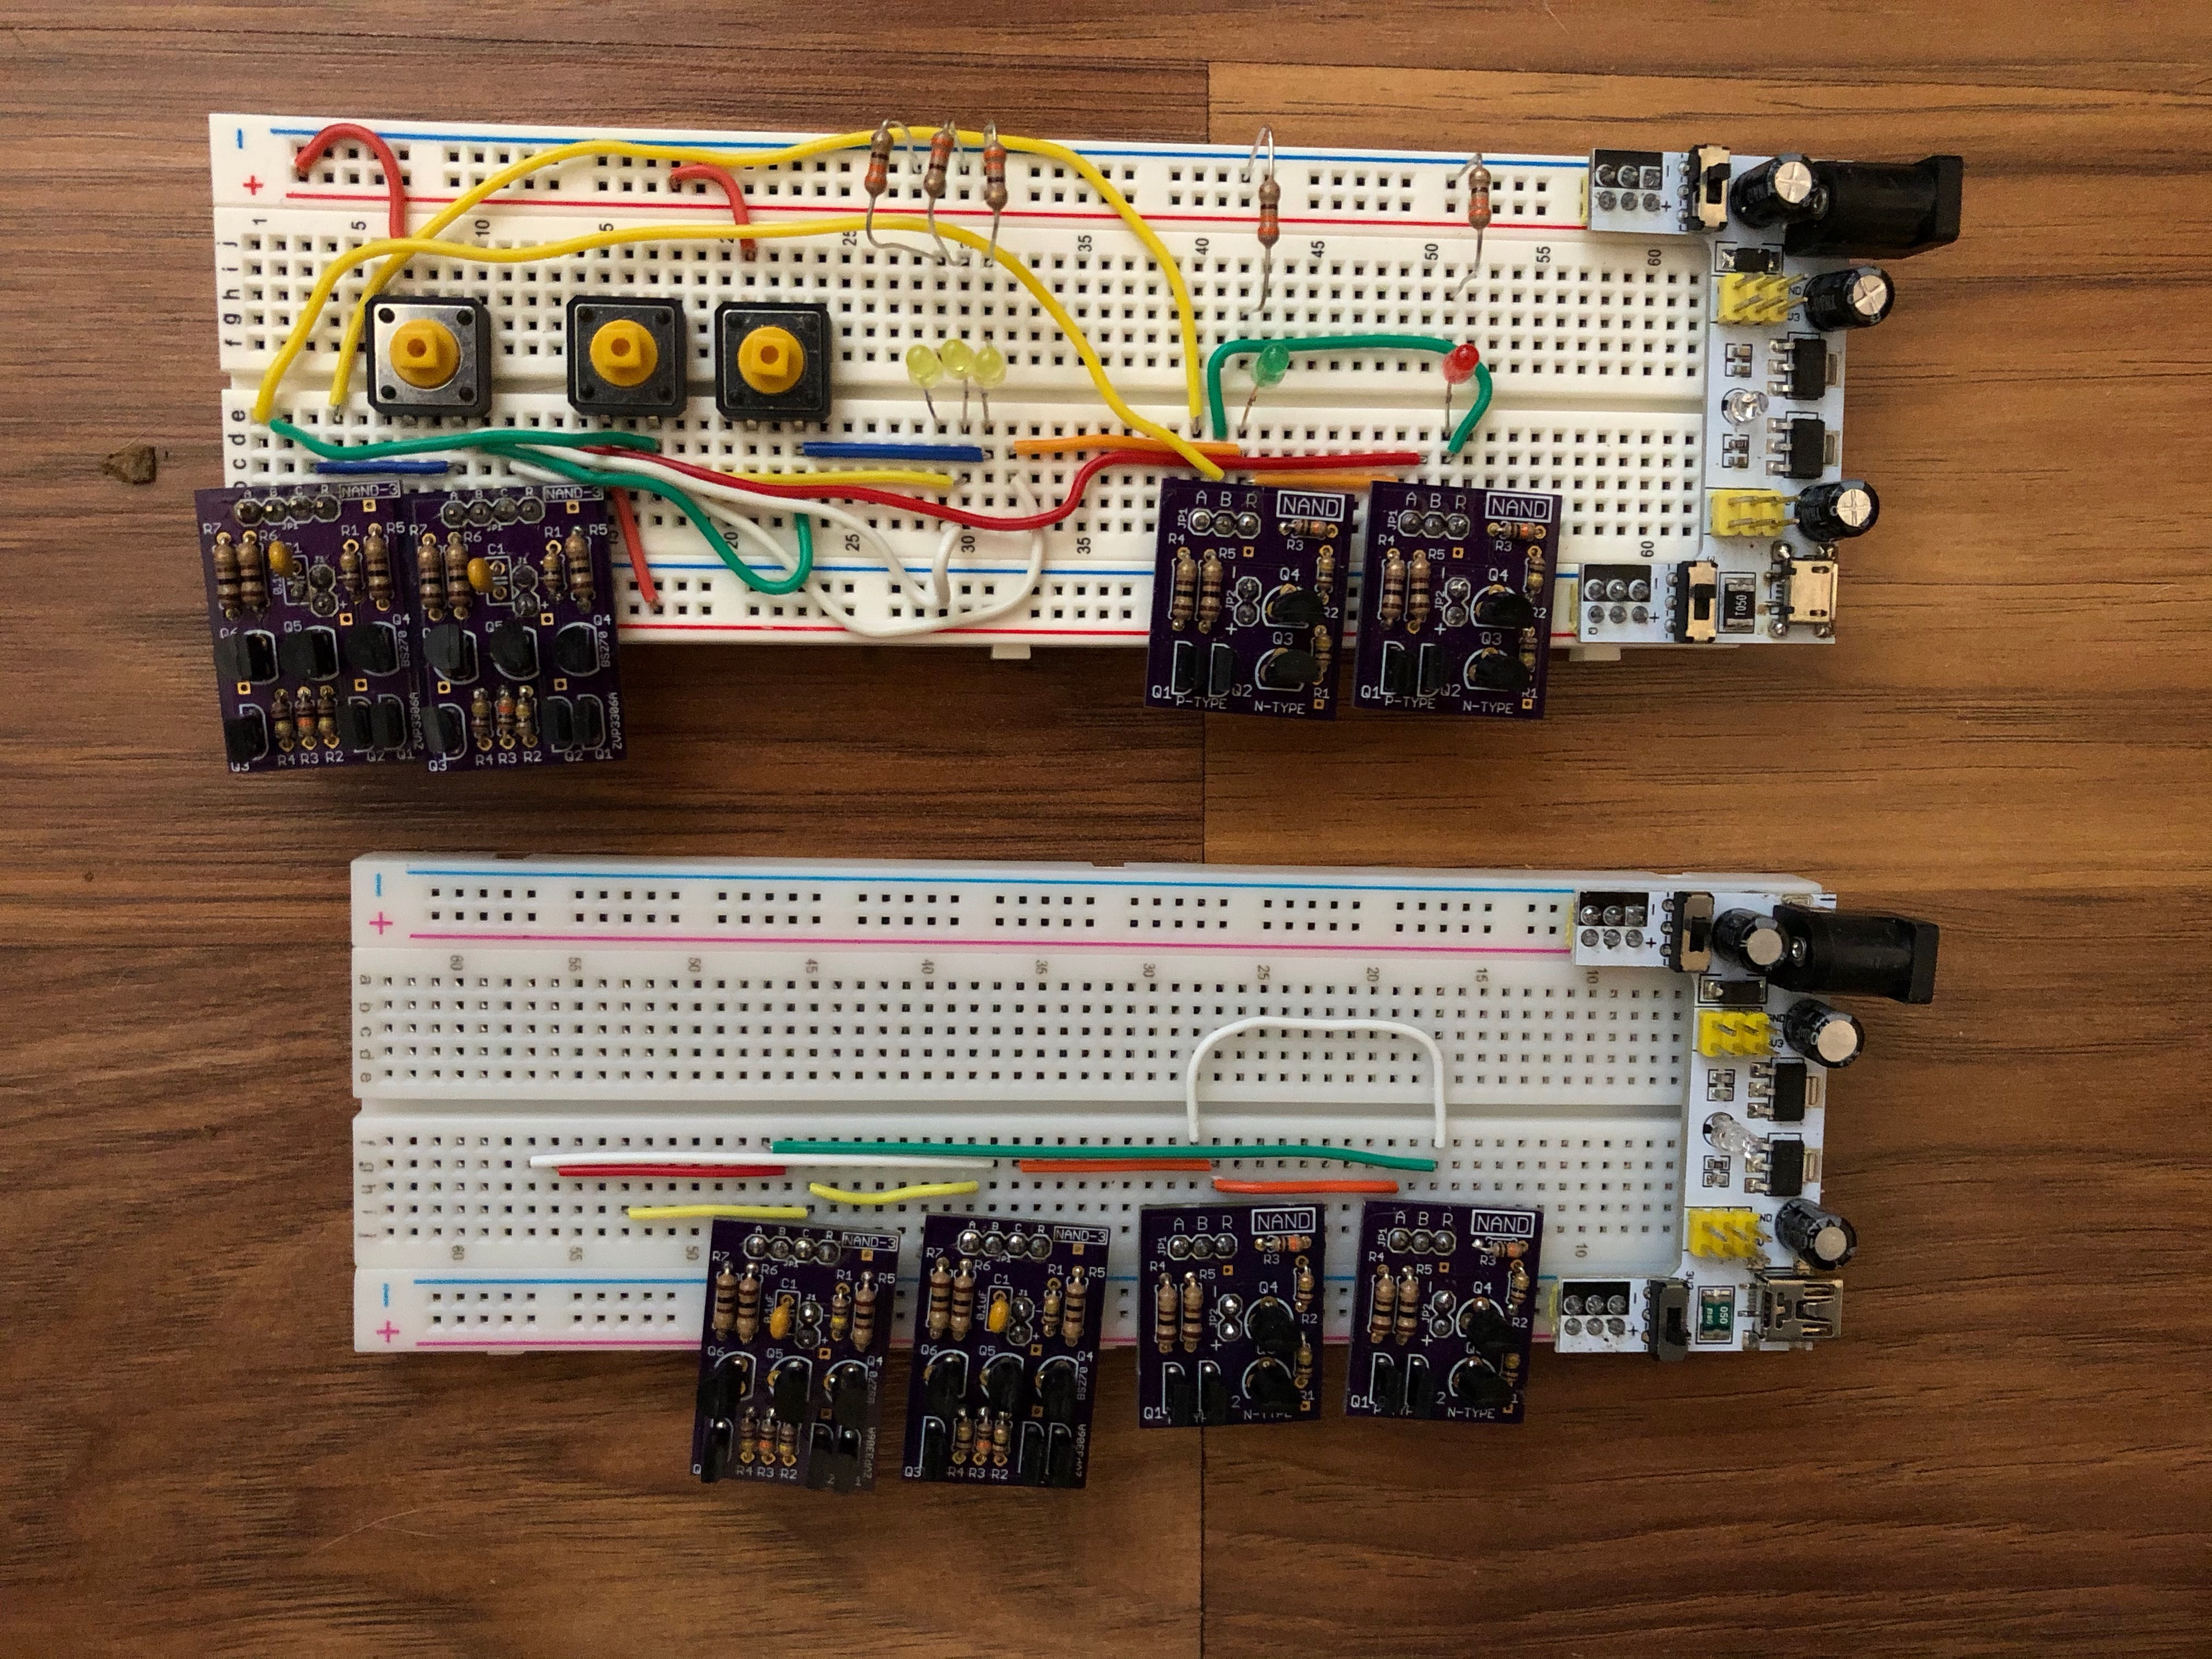
\includegraphics[scale=0.10]{twoflipflops.jpg}
  \caption{Two bits of data storage, using JK flip-flop gates.}
  \end{center}
\end{figure}

